%-------------------------------------------------------
\section{The Crisis}
%-------------------------------------------------------

\begin{frame}

\begin{center}
{\LARGE The Crisis}
\end{center}

\end{frame}

%-------------------------------------------------------

%-------------------------------------------------------

\begin{frame}{Housing market and mortgage debt}

\begin{figure}
\begin{center}

\resizebox{0.70\textwidth}{!}{%
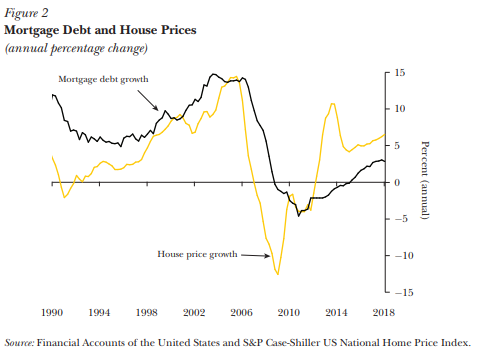
\includegraphics{Figures/aikman_et_al_house_prices_mortage.png}
}

\caption{House prices and mortgage debt. Source: \href{https://pubs.aeaweb.org/doi/pdfplus/10.1257/jep.33.1.107}{Aikman \emph{et al} (2019)}}

\end{center}
\end{figure}

\end{frame}

%-------------------------------------------------------

%-------------------------------------------------------

\begin{frame}{Rapid deterioration of MBS market}

\begin{figure}
\begin{center}

\resizebox{0.38\textwidth}{!}{%
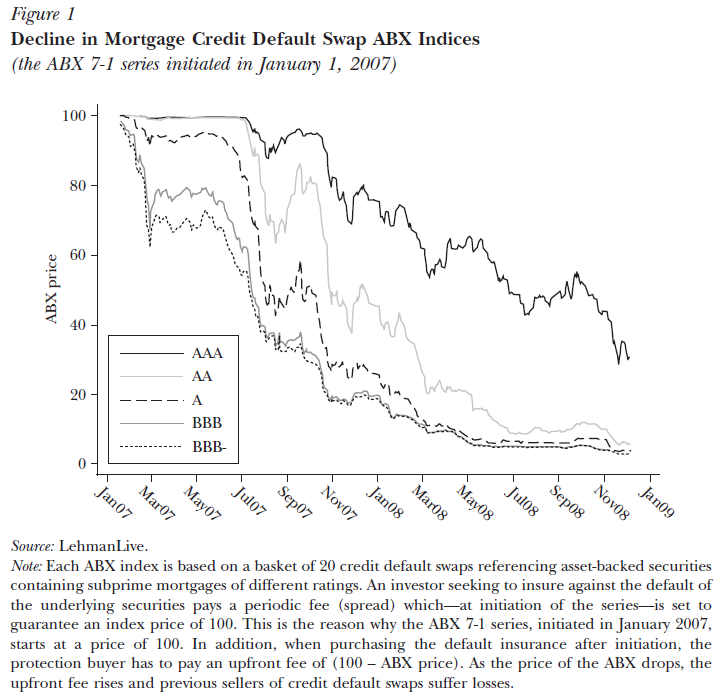
\includegraphics{Figures/ABX_indices.png}
}

\caption{\label{fig:L4_ABX_indices}  Source: \href{https://www.princeton.edu/~markus/research/papers/liquidity_credit_crunch.pdf}{Brunnermeier (2009); Bloomberg}}

\end{center}
\end{figure}

\begin{itemize}
\item	Sudden deterioration in sentiment in MBS markets
\item	Reflects higher (perceived) probabilities of systematic defaults in pools
\item	House-price slowdown and some funds needing parent support
\end{itemize}

\end{frame}

%-------------------------------------------------------

%-------------------------------------------------------

\begin{frame}{Shutdown of asset backed commercial paper markets}

\begin{figure}
\begin{center}

\resizebox{0.55\textwidth}{!}{%
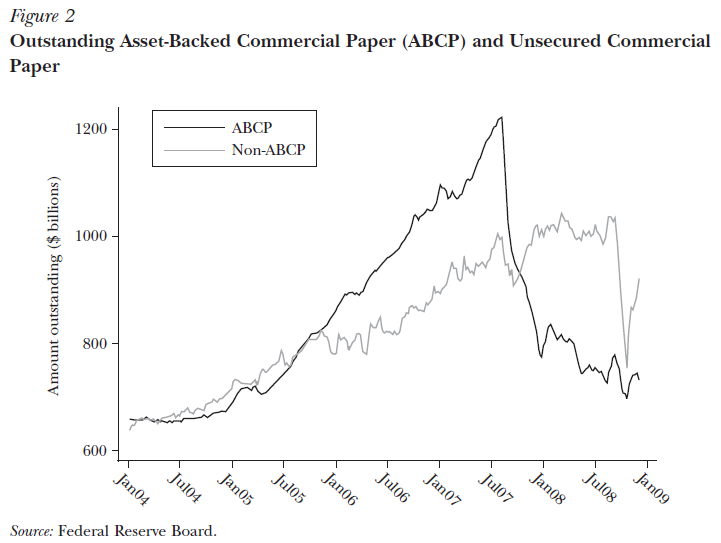
\includegraphics{Figures/ABCP_cliff.png}
}

\caption{\label{fig:L4_ABCP_cliff} Collapse in ABCP (eventually followed by non-asset backed paper). Source: \href{https://www.princeton.edu/~markus/research/papers/liquidity_credit_crunch.pdf}{Brunnermeier (2009); Bloomberg}}

\end{center}
\end{figure}

\begin{itemize}
\item	Note the initial impact is in the \emph{asset backed} segment
\end{itemize}

\end{frame}

%-------------------------------------------------------

%-------------------------------------------------------

\begin{frame}{Fear in the interbank markets}

\begin{figure}
\begin{center}

\resizebox{0.60\textwidth}{!}{%
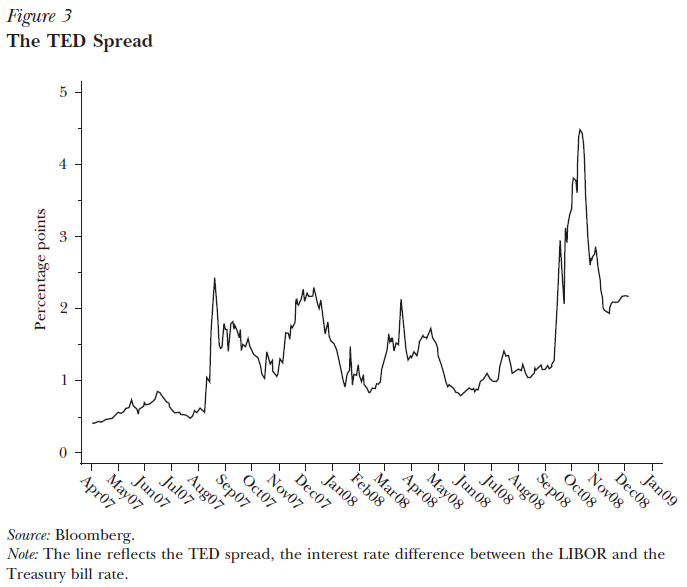
\includegraphics{Figures/ted_spread.png}
}

\caption{\label{fig:L4_ted_spread} Ted spread: 3-Mo LIBOR - 3-Mo T-Bill as a measure of interbank funding difficulties}

\end{center}
\end{figure}

\end{frame}

%-------------------------------------------------------

%-------------------------------------------------------

\begin{frame}{Fear in the interbank markets}

\begin{figure}
\begin{center}

\resizebox{0.80\textwidth}{!}{%
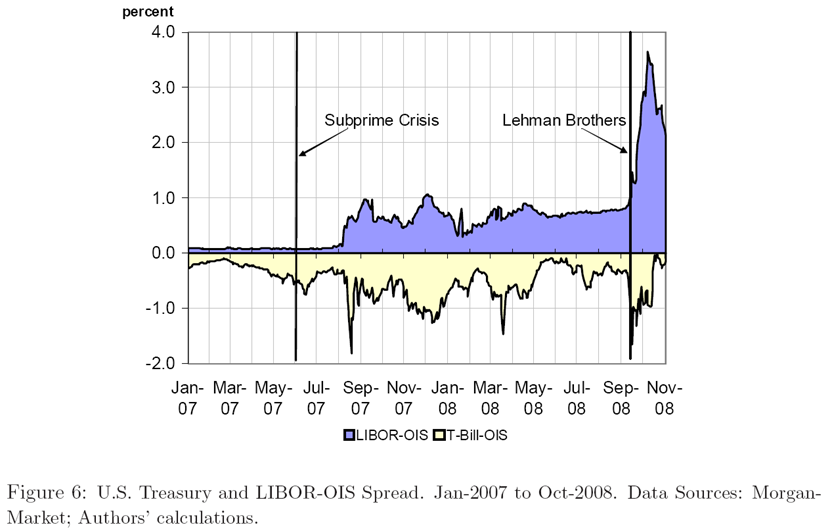
\includegraphics{Figures/caballero_et_al_ted_spread.png}
}

\caption{\label{fig:L4_ted_spread_and_liquidity} Decomposing Ted-spread into `risk' and `liquidity'. Source: Caballero, Fahri and Gourinchas (2008) - also see \href{https://www.investopedia.com/articles/active-trading/061114/what-ois-libor-spread-and-what-it.asp}{here}}

\end{center}
\end{figure}

%Most likely, the strong U.S. capital inflows of the last few years contributed to the significant weakening of U.S. credit markets. The eventual recognition of their degraded performance was one of the triggers of the current crisis. However, this weakening is in itself
%part of the endogenous response of U.S. financial markets to world financial conditions. In
%effect, U.S. assets became stretched by trying to accommodate the world’s excess demand
%for assets. Therein lies the structural problem. This chronic excess demand for assets derives from financial underdevelopment in emerging markets and most commodity producing
%economies, rather than from macroeconomic imbalances. Excess asset demand leaves an
%unmistakable signature in low real interest rates, which in turn provide a fertile ground for
%bubbles to emerge. Thus an alternative –perhaps metaphoric– interpretation of the sequence
%of events is that the bubble located in emerging markets during the 1990s migrated toward
%the U.S. housing and credit markets (and the NASDAQ before that) following the EM crisis
%and the coming on-line of capitalist China.

\end{frame}

%-------------------------------------------------------

%-------------------------------------------------------

\begin{frame}{Fear in the interbank markets}

\begin{figure}
\begin{center}

\resizebox{0.70\textwidth}{!}{%
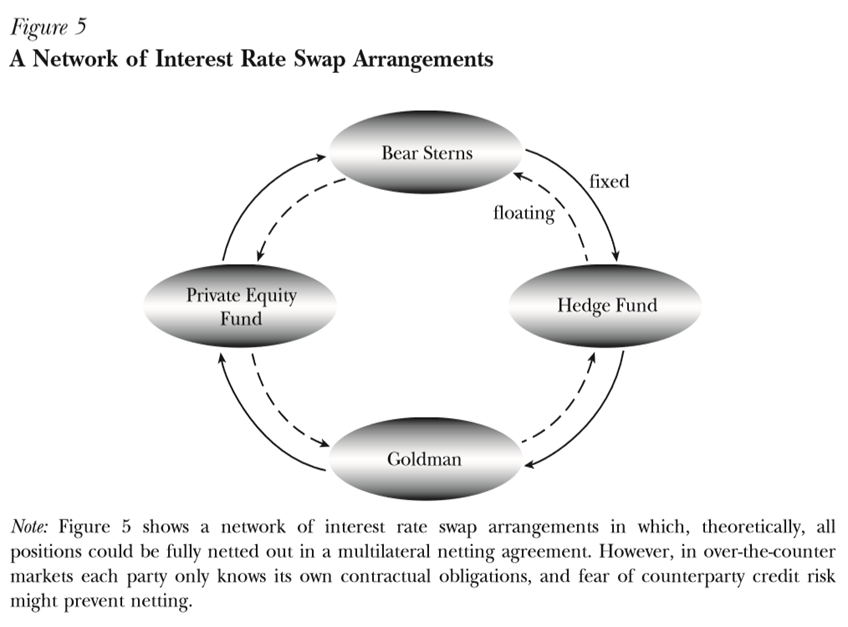
\includegraphics{Figures/swap_net_vs_gross.png}
}

\caption{\label{fig:L4_swap_net_vs_gross} Complexity and opacity of interbank and financial intermediary networks implies netting of positions subject to ambiguity. Source: \href{https://www.princeton.edu/~markus/research/papers/liquidity_credit_crunch.pdf}{Brunnermeier (2009); Bloomberg}}

\end{center}
\end{figure}

\end{frame}

%-------------------------------------------------------

%-------------------------------------------------------

\begin{frame}{Run on repo}

Remember Diamond-Dybvig model of bank runs and the famous movie, \emph{`It's a wonderful life'}\ldots

\end{frame}

%-------------------------------------------------------

%-------------------------------------------------------

\begin{frame}{Run on repo}

\begin{figure}
\begin{center}

\resizebox{0.70\textwidth}{!}{%
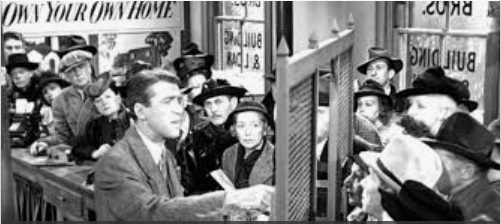
\includegraphics{Figures/its_wonderful.png}
}

\end{center}
\end{figure}

\end{frame}

%-------------------------------------------------------

%-------------------------------------------------------

\begin{frame}{Run on repo}

\ldots or \emph{`Mary Poppins'}\ldots

\end{frame}

%-------------------------------------------------------

%-------------------------------------------------------

\begin{frame}{Run on repo}

\begin{figure}
\begin{center}

\resizebox{0.70\textwidth}{!}{%
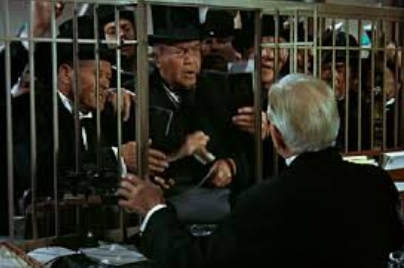
\includegraphics{Figures/mary_poppins_1.png}
}

\end{center}
\end{figure}

\end{frame}

%-------------------------------------------------------

%-------------------------------------------------------

\begin{frame}{Run on repo}

\begin{figure}
\begin{center}

\resizebox{0.70\textwidth}{!}{%

\includegraphics{Figures/mary_poppins_2.png}
}

\end{center}
\end{figure}

\end{frame}

%-------------------------------------------------------

%-------------------------------------------------------

\begin{frame}{Run on repo}

\begin{quote}
What happened is analogous to the banking panics of the 19th century in which depositors \emph{en masse} went to their banks seeking to withdraw cash in exchange of demand and savings deposits. \textbf{The banking system could not honor these demands because the cash had been lent out and the loans were illiquid}, so instead they suspended convertibility and relied on clearinghouses to issue certificates as makeshift currency. Evidence of the insolvency of the banking system in these earlier episodes is the discount on these certificates. \textbf{We argue that the current crisis is similar in that contagion led to `withdrawals' in the form of unprecedented high repo haircuts and even the cessation of repo lending on many forms of collateral.}
\end{quote}
\begin{center}
- Gorton and Metrick (2009)
\end{center}

\end{frame}

%-------------------------------------------------------

%-------------------------------------------------------

\begin{frame}{Run on repo}

Investor buys some asset (acts as collateral) from the bank for $X$
\begin{itemize}
\item	Bank agrees to repurchase the same asset some time later (perhaps the next
day) for $Y$
\item	The percentage (Y-X)/X is the “repo rate” ($\approx$ interest
rate on a bank deposit)
\item	Typically, the total amount of the deposit will be some amount less than the value of the underlying asset (the difference is the `haircut').
\end{itemize}
\vspace{2mm}
Numerical example\ldots
	\begin{itemize}
	\item	An asset has a market value of $100$
	\item	Bank sells it for $80$ with an agreement to repurchase it for $88$
	\item	Repo rate is $10\%$ $\left( \frac{88-80}{80} \right)$
	\item	Haircut is $20\%$ $\left( \frac{100 – 80}{100} \right)$
	\item	If bank defaults on promise to repurchase, the investor keeps collateral
	\end{itemize}

\end{frame}

%-------------------------------------------------------

%-------------------------------------------------------

\begin{frame}{Run on repo}

Pools of mortgages are used as collateral by SPVs when they borrow
\begin{itemize}
\item	Also, the outputs of securitization (MBS etc.) are \textit{themselves} often used as collateral
\end{itemize}
\vspace{2mm}
Haircut plays the role of reserves (covering a fraction of deposits) in the traditional model of banking
	\begin{itemize}
	\item	Forces bank to keep some fraction of their assets in reserve
	\item	Note this captures a form of `solvency' protection
	\end{itemize}
\vspace{2mm}
Collateral plays the role of (govt-provided) deposit insurance in traditional model of banking
\begin{itemize}
\item	Maintains faith of lender
\item	What what if collateral starts to be questioned?
\end{itemize}

\end{frame}

%-------------------------------------------------------

%-------------------------------------------------------

\begin{frame}{Run on repo}

\begin{figure}
\begin{center}

\resizebox{0.70\textwidth}{!}{%
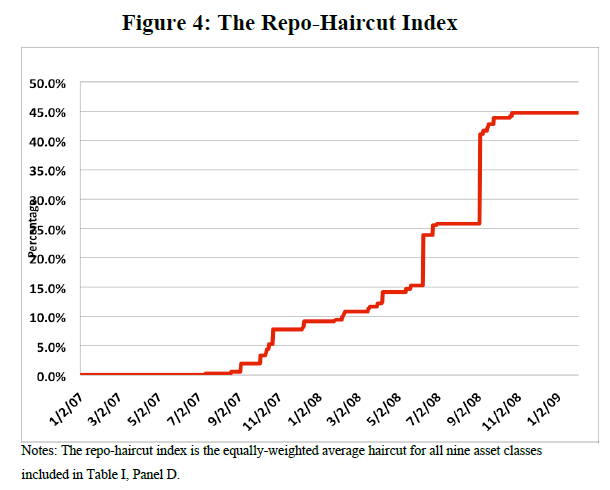
\includegraphics{Figures/gorton_metrick_repo_haircut.png}
}

\caption{\label{fig:L4_gorton_metrick_repo_haircut} Repo haircut - averaged over asset classes. Source: Gorton and Metrick (2009)}

\end{center}
\end{figure}

\end{frame}

%-------------------------------------------------------

%-------------------------------------------------------

\begin{frame}{Run on repo}

Numerical example of effects of haircut $\uparrow$
	\begin{itemize}
	\item	Suppose repo market size $= 10$
	\item	Haircut of $0\%$ $\Rightarrow$ banks can raise financing of $10$
	\item	Suppose haircut rises to $20\%$ on average
	\item	Then banks can only raise $8$ in financing
	\item	Need to find other ways - new securities? Difficult.
	\item	May need to sell assets - but this might drive prices down and will typically be the assets used as collateral!
	\item	This hampers them further as raises more concern about solvency - leading to higher haircuts\ldots
	\end{itemize}
\vspace{2mm}
Additionally, the size of the potential market might shrink
\begin{itemize}
\item	Money market funds leaving the market
\end{itemize}

\end{frame}

%-------------------------------------------------------

%-------------------------------------------------------

\begin{frame}{Crisis timeline}

There are useful timelines of the crisis online (I here summarize)
	\begin{itemize}
	\item	\href{https://www.stlouisfed.org/financial-crisis/full-timeline\#2008}{St Louis Fed}
	\item	\href{https://www.thebalance.com/2007-financial-crisis-overview-3306138}{2007}, \href{https://www.thebalance.com/2008-financial-crisis-timeline-3305540}{2008} and \href{https://www.thebalance.com/2009-financial-crisis-bailouts-3305539}{2009} from `The Balance' website
	\end{itemize}
\vspace{3mm}
See, also, the timelines provided in \href{https://www.princeton.edu/~markus/research/papers/liquidity_credit_crunch.pdf}{Brunnermeier (2009)} and, more recently, in \href{https://pubs.aeaweb.org/doi/pdfplus/10.1257/jep.33.1.107}{Aikman \emph{et al} (2019)}

\end{frame}

%-------------------------------------------------------

%-------------------------------------------------------

\begin{frame}{Crisis timeline - 2007}

\textbf{Early 2007}
	\begin{itemize}
	\item	Home sales/prices peak and troubles emerge in MBS and funds invested in them
	\item	New Century Financial `death spiral' (subprime lender), Bear Stearns suspended redemptions from a prominent fund, ratings downgrades on swathes of MBS
	\end{itemize}
\vspace{2mm}
\textbf{Summer}
	\begin{itemize}
	\item	Housing market numbers continued to worsen and, in late Summer, interbank lending was stressed (recall Ted spread discussion)
	\item	Fed cuts rate by 50bp in August to 4.75 (would be 4.25 by year-end)
	\item	American Home Mortgage Investment Corporation goes bankrupt
	\item	BNP Paribas halts redemptions on mortgage/MBS related funds
	\end{itemize}
\vspace{2mm}	
\textbf{Fall}
	\begin{itemize}
	\item	Housing market continues to weaken
	\item	Northern Rock (old-skool) run in the UK
	\end{itemize}

\end{frame}

%-------------------------------------------------------

%-------------------------------------------------------

\begin{frame}{Crisis timeline - 2007}

\textbf{December}
	\begin{itemize}
	\item	Transmission of monetary policy (rate cuts) was not freeing up bank lending as spreads over safe rates were widening
	\item	To avoid stigma of discount window lending, Fed creates Term Auction Facility
		\begin{itemize}
		\item	Provides collateralized (even with various MBS) funding to banks with sub-prime exposures
		\item	Trying to follow Bagehot approach
		\item	Like an anonymous discount window
		\item	Intended to give breathing room - avoid firesale into closed/dislocated markets
		\end{itemize}
	\item	Foreclosures pick up speed - but problems still largely restricted to financial markets, banking system and housing market (not broader economy, yet)
	\end{itemize}

\end{frame}

%-------------------------------------------------------

%-------------------------------------------------------

\begin{frame}{Crisis timeline - 2007}

\begin{quote}
Under the Term Auction Facility (TAF) program, the Federal Reserve will auction term funds to depository institutions against the wide variety of collateral that can be used to secure loans at the discount window.  All depository institutions that are judged to be in generally sound financial condition by their local Reserve Bank and that are eligible to borrow under the primary credit discount window program will be eligible to participate in TAF auctions.  All advances must be fully collateralized.  By allowing the Federal Reserve to inject term funds through a broader range of counterparties and against a broader range of collateral than open market operations, this facility could help promote the efficient dissemination of liquidity when the unsecured interbank markets are under stress.
\end{quote}

\end{frame}

%-------------------------------------------------------

%-------------------------------------------------------

\begin{frame}{Crisis timeline - 2008}

\textbf{Early 2008}
	\begin{itemize}
	\item	Fed continues cutting
	\item	Tax rebates announced (though not to be paid until summer)
	\item	But housing market and foreclosures keep worsening
	\item	BoA buys Countrywide (aggressive subprime lender) and Ambac Financial Group downgraded (important guarantor / monoline insurer)
	\end{itemize}
\vspace{2mm}
\textbf{March}
	\begin{itemize}
	\item	Fed extends TAF and other lending facilities
		\begin{itemize}
		%\item	Provide banks holding MBS and CDOs with `good' assets collateral they could then use for funding
		\item	\textbf{Note these are liquidity policies}
		\end{itemize}
	\item	Bear `failure' - acquisition by J. P. Morgan Chase
		\begin{itemize}
		\item	JPMC agreed to pay \$2 a share ($<7\%$ of price two days earlier)
		\item	Partly backed by Fed but JPMC had a first loss position (junior loan)
		\end{itemize}
	\item	Loosening by Fed and opened discount window to investment banks via `Primary Dealer Credit Facility'
		\begin{itemize}
		\item	Overnight funding to investment banks
		\item	Helped Lehman, for now\ldots
		\end{itemize}
	\end{itemize}

\end{frame}

%-------------------------------------------------------

%-------------------------------------------------------

\begin{frame}{Crisis timeline - 2008}

\textbf{Spring-Summer}
	\begin{itemize}
	\item	Further emergency lending by Fed
	\item	Indymac failure
	\item	Housing and Economic Recovery Act allowed Treasure to guarantee some loans backed by Fannie and Freddie (GSEs that securitized huge fraction of U.S. mortgages)
	\item	Discussions about possible future support for the GSEs
	\end{itemize}

\textbf{September}
	\begin{itemize}
	\item	Fannie and Freddie put into conservatorship
		\begin{itemize}
		\item	Made explicit and formalized government backing of the GSEs that had previously been assumed (allowed them to be aggressive in expansion)
		\item	\textbf{Note the similarity to deposit insurance and other moral hazard examples}
		\end{itemize}
	\item	Lehman Brothers failure
		\begin{itemize}
		\item	Had been an attempt to form a private sector buyout
		\item	But Korean SWF, Barclays and BoA backed off (BoA buys Merrill)
		\item	Debate over why Fed `allowed' Lehman to fail\ldots
		\end{itemize}
	\end{itemize}

\end{frame}

%-------------------------------------------------------

%-------------------------------------------------------

\begin{frame}{Crisis timeline - 2008}

Brief aside on Lehman failure
	\begin{itemize}
	\item	Highly levered (less restricted by regulation since not depository institution)
	\item	Short term funding
	\item	Highly exposed to housing market directly and through complex derivatives/MBS
	\item	Had to take big write-downs - especially in subprime (weakening capital position)
	\item	Tried to delever and raise funding but opacity of assets and suspicion in market hindered this
	\item	Once private sector bailout failed and (according to the Fed) it was decided that Lehman had inadequate collateral to secure a loan from the Fed with sufficient certainty that the Fed would not take a loss
	\end{itemize}

\end{frame}

%-------------------------------------------------------

%-------------------------------------------------------

\begin{frame}{Crisis timeline - 2008}

Ball (2018) argues that the Fed's claim that they could not legally provide a loan, was false and not the real reason
	\begin{itemize}
	\item	Implies it was a political decision to avoid moral hazard (driven by Paulson)
	\item	Claims there were plenty of assets that, even conservatively valued, could have secured a loan to allow at least an orderly wind-down (avoiding value destruction that certainly did occur in the chaos)
	\item	Should have helped as they helped Bear and, soon after, helped AIG
	\item	Hadn't realized that the effects would be so disruptive (Bernanke strongly disagrees)
	\end{itemize}
\end{frame}

%-------------------------------------------------------

%-------------------------------------------------------

\begin{frame}{Crisis timeline - 2008}

Great reference to understand `How big banks fail' is Duffie's book of that title
\begin{itemize}
\item	Here I quickly summarize his description of the stages of a `typical' failure (of a big dealer bank - see Bear, Lehman)
\item	This and the (more difficult) Ball book are very useful for getting a grip on the nuts and bolts of how these banks functioned before the crisis (without endorsing Ball's take on why Lehman was `allowed' to fail)
\item	You won't be tested on minute details of these books - but they're good reads if you're interested in this world\ldots
\end{itemize}

\end{frame}

%-------------------------------------------------------

%-------------------------------------------------------

\begin{frame}{How a big bank fails}


\begin{quote}
Dealer banks are financial institutions that intermediate the `backbone' markets for securities and over-the-counter (OTC) derivatives. These activities tend to be bundled with other
wholesale financial market services, such as prime brokerage and underwriting. Because of
their size and their central position in the plumbing of the financial system, the failure of
a dealer bank could place significant stress on its counterparties and clients, and also on
the prices of assets or derivatives that it holds. The collapse of a major dealer bank also
reduces the ability of the financial system to absorb further losses and to provide credit and
liquidity to major market participants. Thus, the potential failure of a major dealer bank is
a systemic risk.
\end{quote}
\begin{center}
- Duffie, \emph{How big banks fail - and what to do about it}, 2011
\end{center}

\end{frame}

%-------------------------------------------------------

%-------------------------------------------------------

\begin{frame}{How big banks fail}

\begin{figure}
\begin{center}

\resizebox{0.90\textwidth}{!}{%
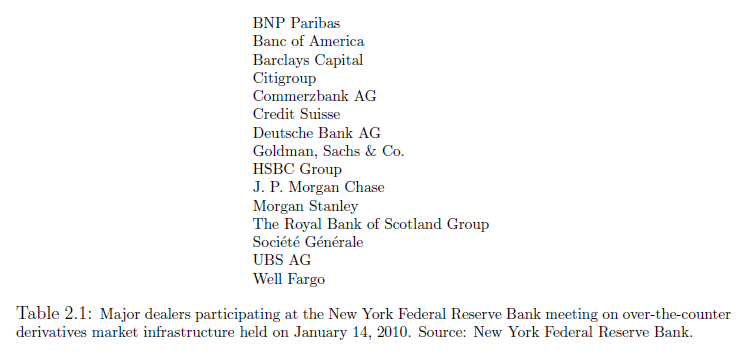
\includegraphics{Figures/dealer_banks.png}
}

\end{center}
\end{figure}

\end{frame}

%-------------------------------------------------------

%-------------------------------------------------------

\begin{frame}{How a big bank fails}

Suppose something (MBS?) has happened to cause substantial losses or drains on liquidity for bank, `Beta'
	\begin{itemize}
	\item	Hasn't devastated the bank but has weakened its position notably	
	\end{itemize}
\vspace{2mm}
Bank tries to signal strength and protect franchise value by not scaling back, but `putting on a brave face'
	\begin{itemize}
	\item	To prevent loss of counterparties and clients they bail out clients on investments arranged by Beta and continue to offer them good terms (e.g. implicit backing for off balance sheet SPVs)
	\item	But this drains funds (which in the future will be a problem)
	\end{itemize}


\end{frame}

%-------------------------------------------------------

%-------------------------------------------------------

\begin{frame}{How a big bank fails}

Confidence dented $\Rightarrow$ counterparties are avoiding Beta/reducing positions
	\begin{itemize}
	\item	Might need to top up their collateral / satisfy margin calls
	\item	Other dealers may be asked to step in between Beta and its counterparties (novations)
	\item	Rumours spread as dealers become wary of increasing \emph{their} positions
	\end{itemize}
\vspace{0.5mm}
Beta also has a prime-brokerage business for hedge fund clients, say
	\begin{itemize}
	\item	Provides IT, trade execution, accounting reports
	\item	Vitally, also custodian services - keeps the HF's cash and securities
	\item	HF start to ask for them back to shift them to other dealers
	\item	Can't really say no or rumours become a clamour
	\item	Damages franchise value (this was profitable) eroding attractiveness for investors further - vicious circle
	\item	Note also, the HF securities were frequently used by Beta \emph{on its own behalf} in repo borrowing as collateral - so double/triple whammy
	\end{itemize}

\end{frame}

%-------------------------------------------------------

%-------------------------------------------------------

\begin{frame}{How a big bank fails}

Even \textit{secured} creditors start backing away (disaster)
	\begin{itemize}
	\item	Even if collateral is thought solid, why bother getting involved in admin around default?
	\item	They themselves may need funds and collateral back quickly
	\item	Haircuts also might no longer be though adequate (will they be able to sell collateral for enough even if they get it back?)
	\end{itemize}
\vspace{2mm}
A lot of these loans are repo (recall Gorton) and \textbf{a lot} is rolled over every night
	\begin{itemize}
	\item	If reluctance to lend occurs, the impacts are rapid (recall our discussion last week of shortening of maturity of debt, pre-crisis)
	\item	Must find a lot more funding - especially as haircuts are rising
	\item	Or start selling - but assets are opaque and possibly already underpriced!
	\end{itemize}

\end{frame}

%-------------------------------------------------------

%-------------------------------------------------------

\begin{frame}{How a big bank fails}

Banks need to hold enough cash/securities in clearing accounts
	\begin{itemize}
	\item	Usually only need to average out over the day - intraday credit from clearing banks
	\item	But clearing banks don't want to be left holding the can either
	\item	Removal of intraday credit is the endgame
	\item	Can't execute trades - dead\ldots
	\item	Declare bankruptcy
	\end{itemize}
\end{frame}

%-------------------------------------------------------

%-------------------------------------------------------

\begin{frame}{How big banks fail}

\begin{figure}
\begin{center}

\resizebox{0.60\textwidth}{!}{%
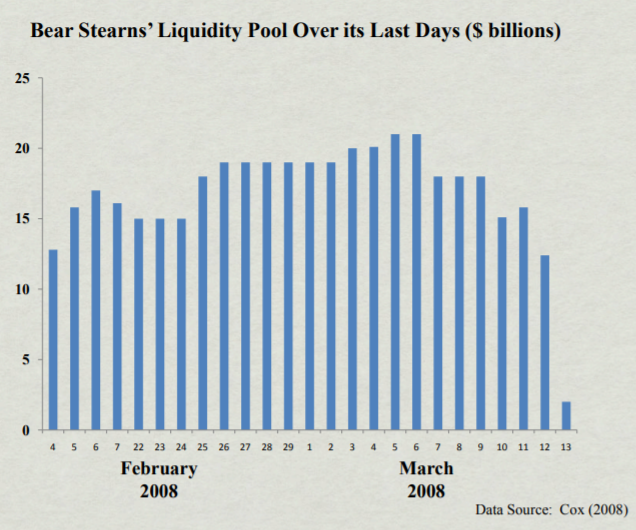
\includegraphics{Figures/bear_stearns_liquidity.png}
}

\end{center}
\end{figure}

\end{frame}

%-------------------------------------------------------

%-------------------------------------------------------

\begin{frame}{Crisis timeline - 2008}

\textbf{Back to September 2008}
	\begin{itemize}
	\item[]	Fed buys AIG
		\begin{itemize}
		\item	Had used their profitable \emph{core} insurance business to fund a business insuring mortgage/mortgage derivative positions - including insuring securities
		\item	Was hugely interconnected via this insurance
		\item	If they failed, the insurance would vanish, causing huge losses across swathes of investors and further asset price declines
		\item	AIG avoided a disruptive bankruptcy but shareholders were wiped out and replaced with Treasury preferred shares etc. after Fed initially made loans (contrast with Lehman)
		\end{itemize}
	\end{itemize}

\end{frame}

%-------------------------------------------------------

%-------------------------------------------------------

\begin{frame}{Crisis timeline - 2008}

\textbf{Still September 2008 - not a good month}
	\begin{itemize}
	\item[]	Reserve Primary Fund broke the buck and broader MMF problems
		\begin{itemize}
		\item	Partly from direct exposure to Lehman (RPF) - also from general contagion and concern at their holdings
		\item	\textbf{Any sniff of risk in these funds and depositors would pull out (they had previously been thought to be riskless - like money)}
		\item	\textcolor{red}{\textbf{MMF unable to finance themselves would pull back on CP holdings which is lifeblood of corp America for working capital}}
		\item	Fed insurance of MMF via `Asset-backed CP MMF Liquidity Facility'
		\end{itemize}
\vspace{1mm}
\item[]	Goldman and MS become commercial banks
	\begin{itemize}
	\item	Can access discount window
	\item	\textbf{No more investment banks on Wall Street!}
	\end{itemize}
\vspace{1mm}
\item[]	WaMu bankrupt after `silent' run
	\begin{itemize}
	\item	Handled by FDIC and sold to JPMC
	\item	Also, Wachovia bought by Wells
	\end{itemize}
\vspace{1mm}
\item[]	Treasury requests $\$700bn$ fund from Congress
	\begin{itemize}
	\item	Defeated despite protections for taxpayer and restrictions on banks
	\item	DJ plunges 770 points
	\end{itemize}
	\end{itemize}

\end{frame}

%-------------------------------------------------------

%-------------------------------------------------------

\begin{frame}{Crisis timeline - 2008}

\textbf{Autumn}
	\begin{itemize}
	\item[]	Bill eventually passed on second attempt
		\begin{itemize}
		\item	Emergency Economic Stabilization Act
		\item	Funded `Troubled Asset Relief Program' (TARP)\ldots
		\item	Helped with Capital Purchase Program (injecting funds into banks with stock purchases - i.e. `bailouts' though doesn't imply a loss for taxpayer)
		\item	Additionally - used for AIG, autos companies, `Term Asset-Backed Securities Loan Facility (TALF) and some homeowner refi programs
		\item	Bill also increased salary oversight (surprisingly effective), FDIC insurance limit and suspended some mark to market accounting requirements (response to firesales)
		\end{itemize}
	\vspace{2mm}
	\item[]	Wheels started to come off stock markets around the world
		\begin{itemize}
		\item	Coordinated rate cuts by central banks in response (\textbf{rapidly approaching ZLB})
		\end{itemize}
	\vspace{2mm}
	\item[]	Fed started `Commerical Paper Funding Facility'
		\begin{itemize}
		\item	Buying commerical paper from \textit{highly rated} firms (\textit{even they} couldn't access CP markets)
		\end{itemize}
	\end{itemize}
	
\end{frame}

%-------------------------------------------------------

%-------------------------------------------------------

\begin{frame}{Crisis timeline - 2008}

\textbf{Autumn}
	\begin{itemize}
	\item	Fed set up Money Market Investor Funding Facility
		\begin{itemize}
		\item	To take assets off money market funds and lend them sums to deal with redemptions
		\end{itemize}
	\vspace{2mm}
	\item	Citi receives funding injections
	\vspace{2mm}
	\item	Fed cuts rates to zero
	\vspace{2mm}
	\item	TALF bought debt of non-mortgage securitizers
		\begin{itemize}
		\item	Credit cards, autos, student loans\ldots
		\item	\textbf{Fear of anything securitized had spread!}
		\end{itemize}
	\end{itemize}

\end{frame}

%-------------------------------------------------------

%-------------------------------------------------------

\begin{frame}{Crisis timeline - 2009}

\textbf{February}
	\begin{itemize}
	\item[]	$\$787bn$ economic stimulus package under Obama
		\begin{itemize}
		\item	Homeowner Stability Initiative also launched to help prevent foreclosure
		\item	Revealed that GDP growth was $-6.3\%$ at end of 2008
		\end{itemize}
	\end{itemize}
\vspace{1mm}
\textbf{April}
	\begin{itemize}
	\item[]	Homeowner Affordable Mortgage Program (HARP
		\begin{itemize}
		\item	To promote financing for underwater borrowers
		\item	Rates had fallen but negative equity prevented taking out new mortgages / refi to access them
		\item	Low takeup - by people only slightly underwater - foreclosures continue
		\end{itemize}
	\end{itemize}
\vspace{1mm}
\textbf{October}
	\begin{itemize}
	\item	Unemployment rate reaches $10\%$
	\item	Lending down - loan performance also
	\item	Banks trying to rebuild balance sheets - cuts off credit
	\item	Households trying to rebuild balance sheets - demand declines
	\end{itemize}

\end{frame}

%-------------------------------------------------------

%-------------------------------------------------------

\begin{frame}{Broader effects of the crisis}

So far we've mainly focused on the financial aspects of the crisis
\begin{itemize}
\item	Ultimately, the effect on the broader economy is the most important motivation for reform
\item	We cannot give a complete analysis here
\item	Some of the main channels discussed are\ldots
	\begin{itemize}
	\item	Traditional accelerationist channels through bank weakness and financial market panic
		\begin{itemize}
		\item	Emphasized in Bernanke (2018) in reading list
		\end{itemize}
	\item	Household leverage/debt channel
		\begin{itemize}
		\item	Emphasized by Mian and Sufi (various papers and book)
		\end{itemize}
	\item	Fiscal damage 
		\begin{itemize}
		\item	See recent work by Oscar Jorda \emph{et al}
		\end{itemize}
	\end{itemize}
\end{itemize}

\end{frame}

%-------------------------------------------------------

%-------------------------------------------------------

\begin{frame}{Economic impacts - Housing market}

\begin{figure}
\begin{center}

\resizebox{0.80\textwidth}{!}{%
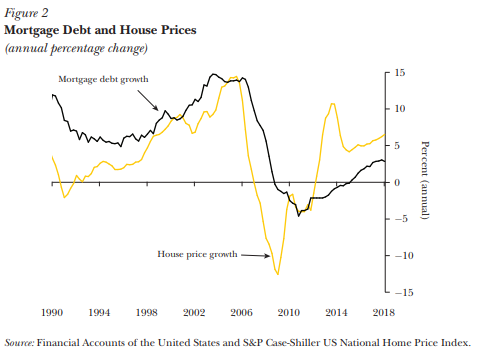
\includegraphics{Figures/aikman_et_al_house_prices_mortage.png}
}

\caption{House prices and mortgage debt. Source: \href{https://pubs.aeaweb.org/doi/pdfplus/10.1257/jep.33.1.107}{Aikman \emph{et al} (2019)}}

\end{center}
\end{figure}

\end{frame}

%-------------------------------------------------------

%-------------------------------------------------------

\begin{frame}{Economic impacts - Household credit problems}

\begin{figure}
\begin{center}

\resizebox{0.80\textwidth}{!}{%
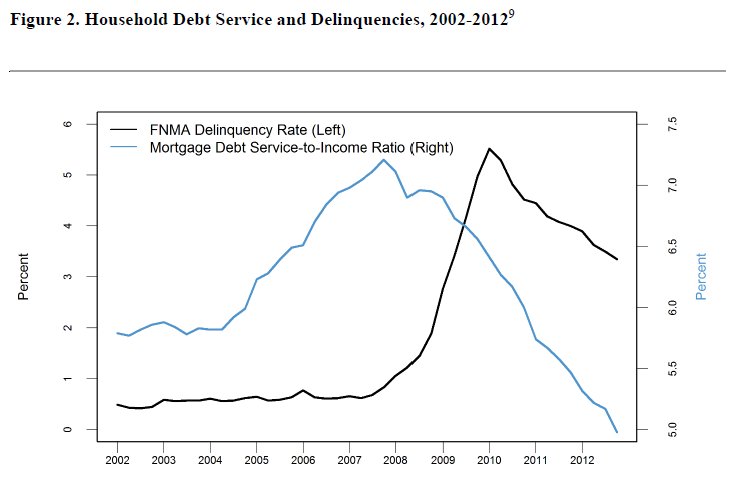
\includegraphics{Figures/dti_and_delinquencies.png}
}

\caption{Household debt to income and delinquencies. Source: Bernanke (2018)}

\end{center}
\end{figure}

\end{frame}

%-------------------------------------------------------

%-------------------------------------------------------

\begin{frame}{Economic impacts - Corporate credit problems}

\begin{figure}
\begin{center}

\resizebox{0.80\textwidth}{!}{%
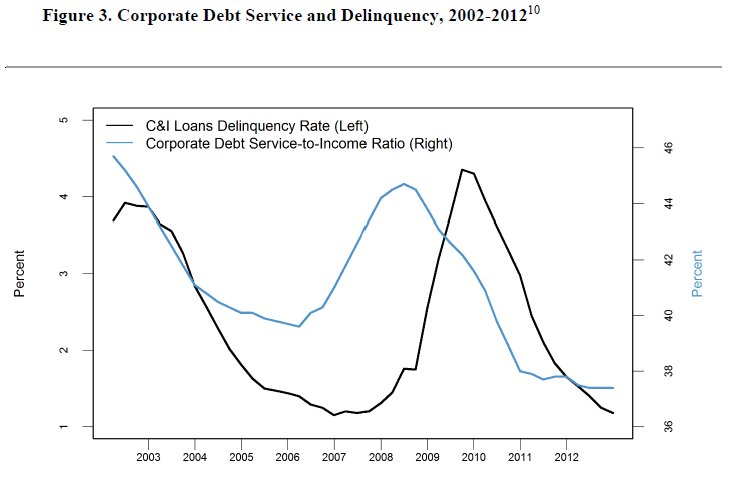
\includegraphics{Figures/corp_loans_delinquency.png}
}

\caption{Corporate debt servicing and delinquencies. Source: Bernanke (2018)}

\end{center}
\end{figure}

\end{frame}

%-------------------------------------------------------

%-------------------------------------------------------

\begin{frame}{Economic impacts - Labor market problems}

\begin{figure}
\begin{center}

\resizebox{0.90\textwidth}{!}{%
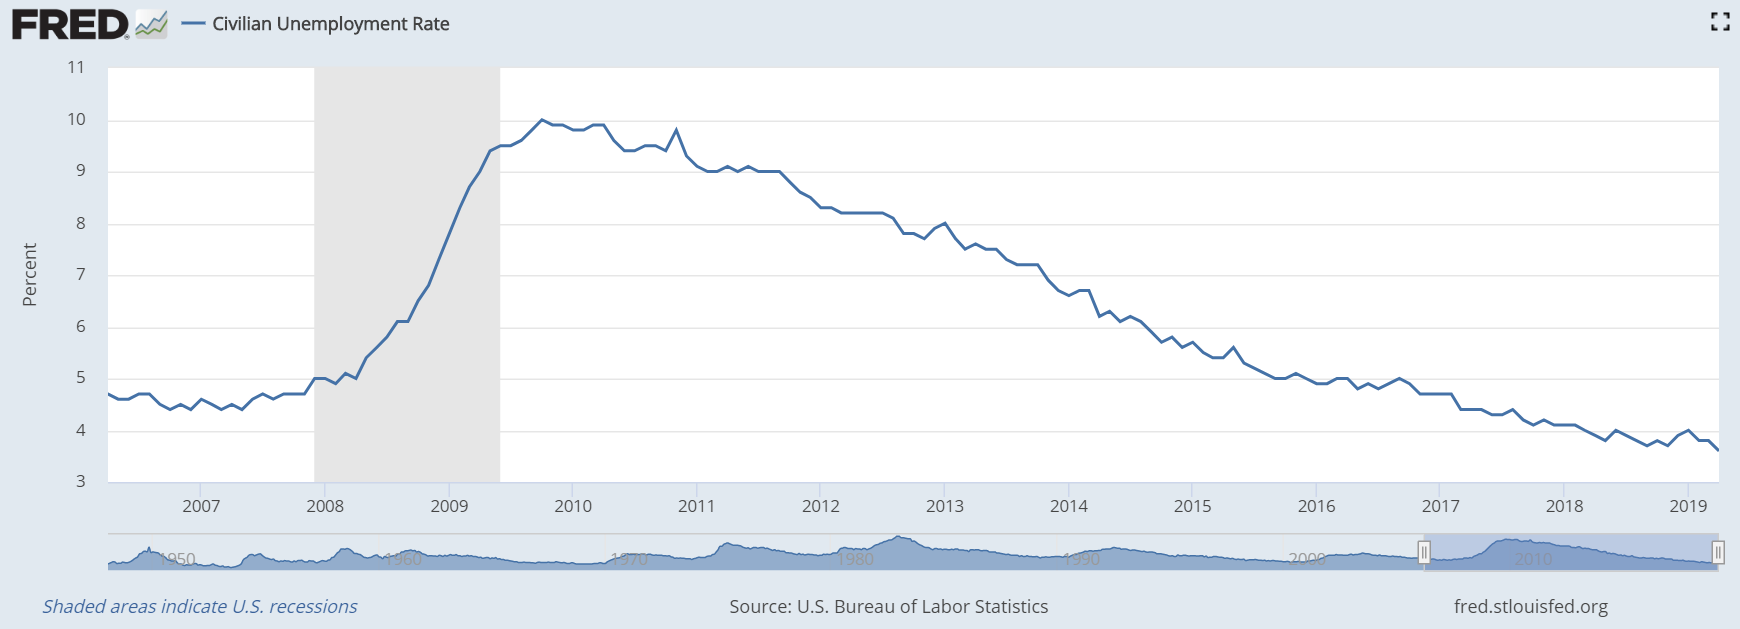
\includegraphics{Figures/unemployment_rate.png}
}

\caption{Unemployment rate. Source: FRED}

\end{center}
\end{figure}

\end{frame}

%-------------------------------------------------------

%-------------------------------------------------------

\begin{frame}{Economic impacts - Deep recession}

\begin{figure}
\begin{center}

\resizebox{0.90\textwidth}{!}{%
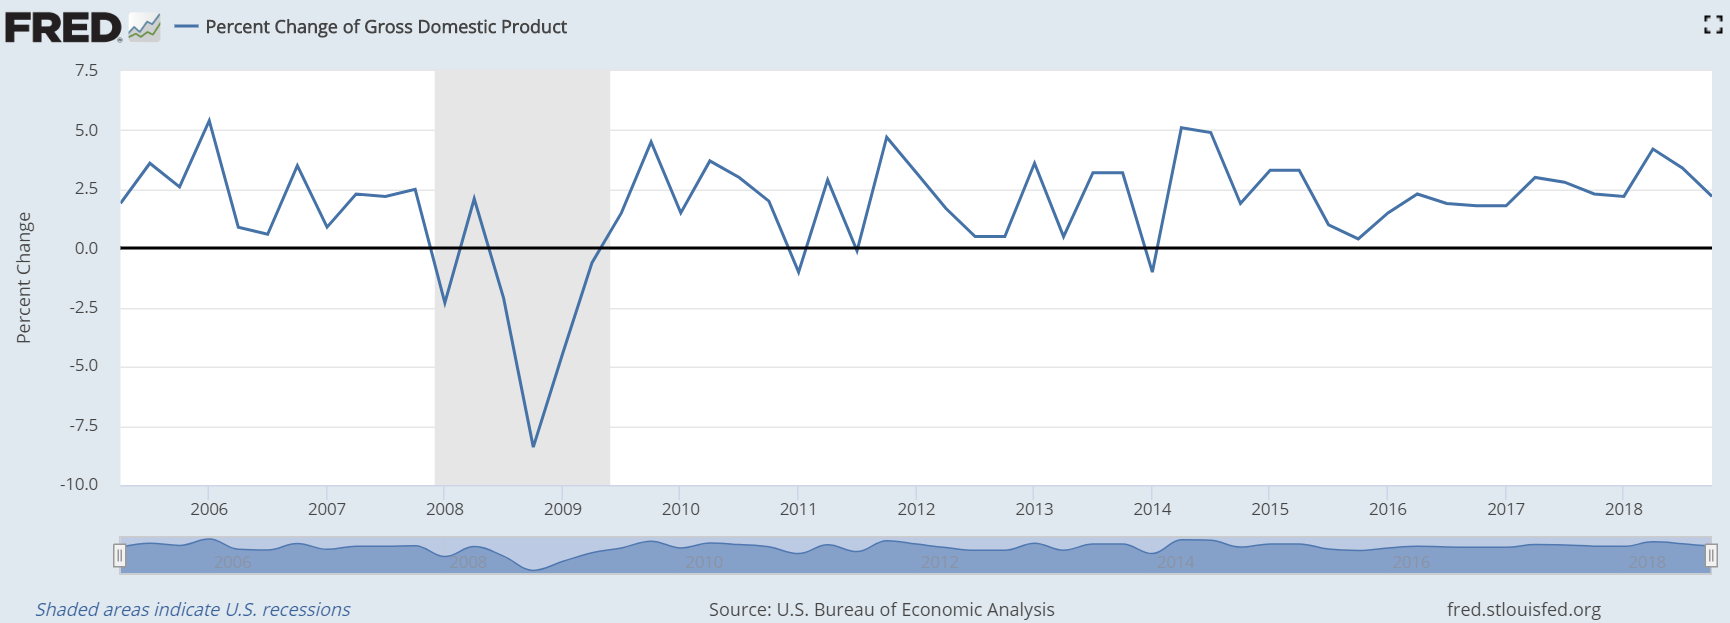
\includegraphics{Figures/recession.png}
}

\caption{Percentage growth in GDP. Source: FRED}

\end{center}
\end{figure}

\end{frame}

%-------------------------------------------------------

%-------------------------------------------------------

\begin{frame}{Economic impacts - Investment off a cliff}

\begin{figure}
\begin{center}

\resizebox{0.90\textwidth}{!}{%
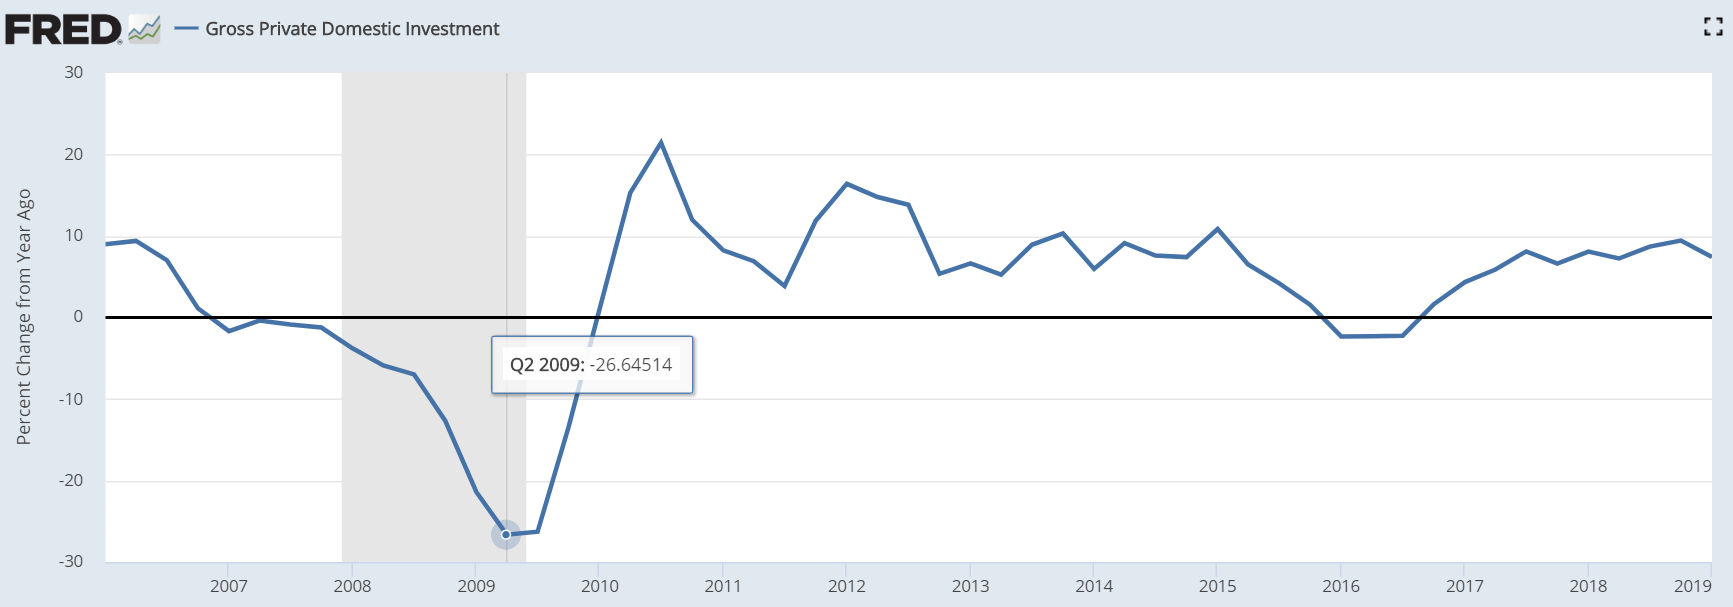
\includegraphics{Figures/investment.png}
}

\caption{Percentage growth YoY in Gross Private Domestic Investment. Source: FRED}

\end{center}
\end{figure}

\end{frame}

%-------------------------------------------------------

%-------------------------------------------------------

\begin{frame}{Economic impacts - Some feedbacks to banks}

\begin{figure}
\begin{center}

\resizebox{0.80\textwidth}{!}{%
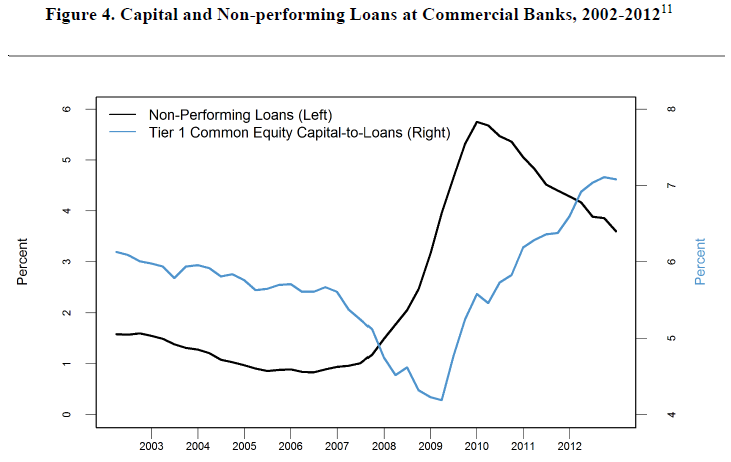
\includegraphics{Figures/npl_commercial_banks.png}
}

\caption{Bad loans grind down bank equity. Source: Bernanke (2018)}

\end{center}
\end{figure}

\end{frame}

%-------------------------------------------------------

%-------------------------------------------------------

\begin{frame}{Broader effects of the crisis}

In the work of Jorda \emph{et al} (various papers) they emphasize that
	\begin{itemize}
	\item	Recessions after \textit{financial} crises are often more prolonged and severe
	\item	A preceding credit bubble is particularly damaging
	\item	Pre-crisis fiscal strength can help mitigate the effects
	\end{itemize}

\end{frame}

%-------------------------------------------------------

%-------------------------------------------------------

\begin{frame}{Slow recovery from Great Recession}

\begin{figure}
\begin{center}

\resizebox{0.65\textwidth}{!}{%
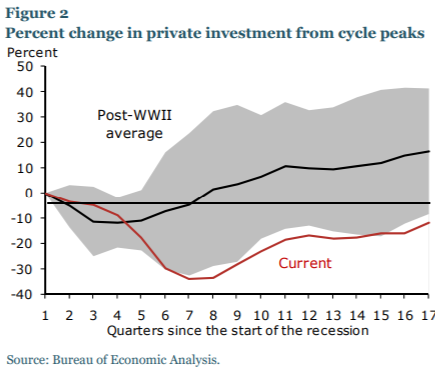
\includegraphics{Figures/investment_av_rec_and_most_recent.png}
}

\caption{Comparing recent and average recovery in investment. Source: Jorda (2012)}

\end{center}
\end{figure}

\end{frame}

%-------------------------------------------------------

%-------------------------------------------------------

\begin{frame}{Slow recovery from Great Recession}

\begin{figure}
\begin{center}

\resizebox{0.65\textwidth}{!}{%
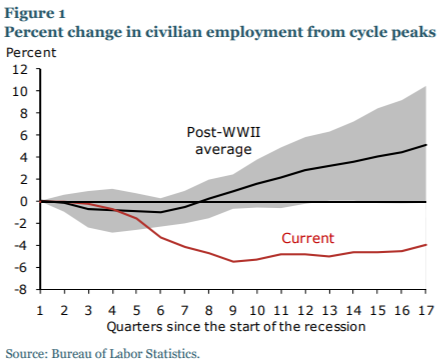
\includegraphics{Figures/unemp_av_rec_and_most_recent.png}
}

\caption{Comparing recent and average recovery in unemployment. Source: Jorda (2012)}

\end{center}
\end{figure}

\end{frame}

%-------------------------------------------------------

%-------------------------------------------------------

\begin{frame}{Fits pattern of recoveries from `financial' recessions}

\begin{figure}
\begin{center}

\resizebox{0.65\textwidth}{!}{%
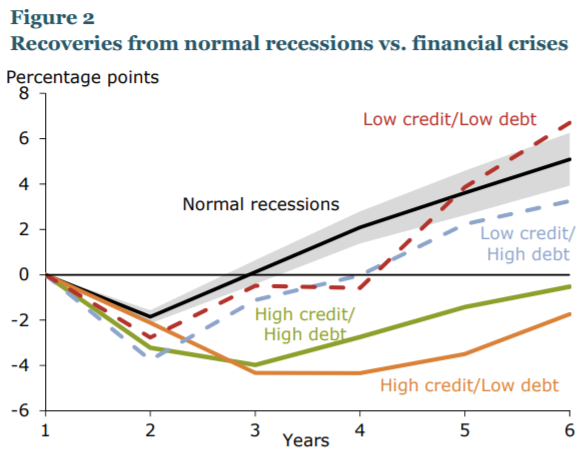
\includegraphics{Figures/recoveries_normal_rec_vs_fin_crises.png}
}

\caption{Comparing recoveries after `normal' and `financial' recessions. Source: Jorda (2012)}

\end{center}
\end{figure}

\end{frame}

%-------------------------------------------------------

%-------------------------------------------------------

\begin{frame}{Importance of public debt}

\begin{figure}
\begin{center}

\resizebox{0.65\textwidth}{!}{%
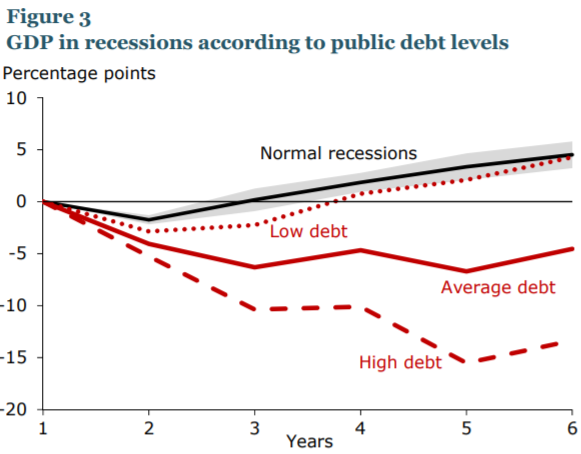
\includegraphics{Figures/recoveries_dependent_on_debt.png}
}

\caption{Comparing recoveries based on initial public debt. Source: Jorda (2012)}

\end{center}
\end{figure}

\end{frame}

%-------------------------------------------------------

%-------------------------------------------------------

\begin{frame}{Economic impacts - GFC damaged fiscal positions}

\begin{figure}
\begin{center}

\resizebox{0.90\textwidth}{!}{%
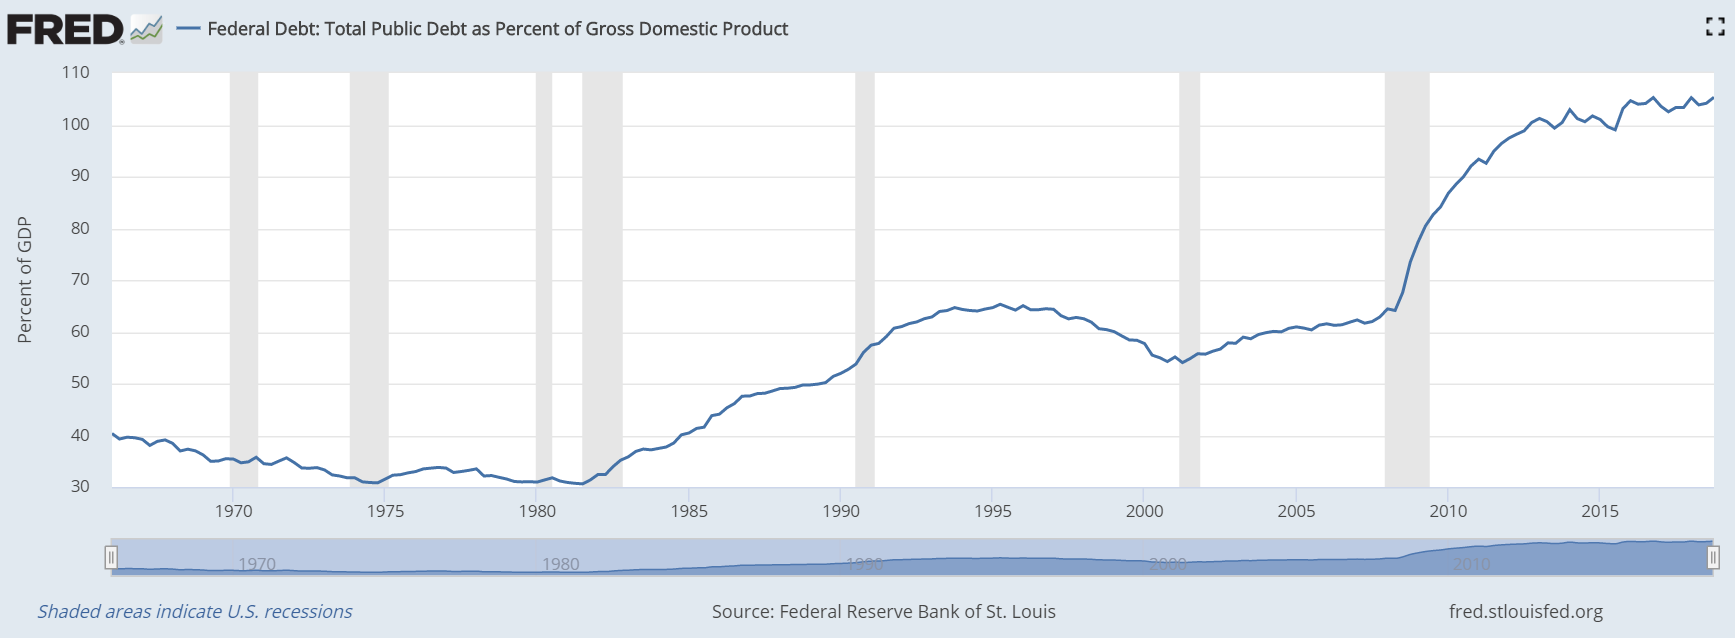
\includegraphics{Figures/debt_to_gdp_US.png}
}

\caption{Dramatic effect on debt levels. Source: FRED}

\end{center}
\end{figure}

\end{frame}

%-------------------------------------------------------

%-------------------------------------------------------

\begin{frame}{Some implications of fiscal damage}

We have concentrated on the US in this section
\begin{itemize}
\item	But the crisis was global
\item	Fiscal damage was widespread, putting, in some cases, immediate restrictions on countercyclical policy or bailouts
	\begin{itemize}
	\item	In some countries banks were both `too big to fail' \textbf{and} too big to save
	\item	Inadequate borrowing ability of governments necessitated austerity
	\item	Even in the U.S. many would argue the large stimulus bill under Obama should have been larger/continued longer
	\end{itemize}
\end{itemize}
\vspace{2mm}
Longer term, it may also imply important reductions in policy flexibility in the `next recession'\ldots
\begin{itemize}
\item	We're still close to ZLB and people question if QE effective
\item	Will fiscal policy be able to step in?
\end{itemize}

\end{frame}

%-------------------------------------------------------

%-------------------------------------------------------

\begin{frame}{But fiscal policy may not be available\ldots}

Ideally, a fiscal expansion can shift the `IS curve' to offset weakness
\begin{itemize}
\item	But, given the damage to fiscal position from GFC and ongoing issues with funding other excessively generous entitlements, will policymakers have enough firepower in the future?
\vspace{3mm}
\end{itemize}
\vspace{2mm}
Might need to rely on unconventional monetary policy and emergency measures again
	\begin{itemize}
	\item	But still controversial and poorly understood
	\item	Legal changes have also tied the Fed's hands in terms of crisis response
	\end{itemize}
\vspace{2mm}
Tricky time for the world economy
\begin{itemize}
\item	Good time for research / new thinking
\item	Go forth\ldots
\end{itemize}

\end{frame}
